\documentclass[12pt]{article}

\usepackage{hyperref} % for auto-linking table of contents
\usepackage{amsmath}
\usepackage[margin=1in]{geometry}
\usepackage{fancyvrb} % fancy verbatim
\usepackage{fancyhdr}
\usepackage{graphicx}
\usepackage{float}
\usepackage{tikz} % for \foreach
\usepackage{caption}
\usepackage{subcaption}

\usepackage{paralist}
\usepackage{listings}
\usepackage{color}

\definecolor{dkgreen}{rgb}{0,0.6,0}
\definecolor{gray}{rgb}{0.5,0.5,0.5}
\definecolor{mauve}{rgb}{0.58,0,0.82}

\lstset{frame=tb,
  language=Matlab,
  aboveskip=3mm,
  belowskip=3mm,
  showstringspaces=false,
  columns=flexible,
  basicstyle={\small\ttfamily},
  numbers=none,
  numberstyle=\tiny\color{gray},
  keywordstyle=\color{blue},
  commentstyle=\color{dkgreen},
  stringstyle=\color{mauve},
  breaklines=true,
  breakatwhitespace=true
  tabsize=3
}


\hypersetup{
    bookmarks=true,         % show bookmarks bar?
    unicode=false,          % non-Latin characters in Acrobat�s bookmarks
    pdftoolbar=true,        % show Acrobat�s toolbar?
    pdfmenubar=true,        % show Acrobat�s menu?
    pdffitwindow=false,     % window fit to page when opened
    pdfstartview={FitH},    % fits the width of the page to the window
    pdftitle={My title},    % title
    pdfauthor={Author},     % author
    pdfsubject={Subject},   % subject of the document
    pdfcreator={Creator},   % creator of the document
    pdfproducer={Producer}, % producer of the document
    pdfkeywords={keyword1} {key2} {key3}, % list of keywords
    pdfnewwindow=true,      % links in new PDF window
    colorlinks=true,       % false: boxed links; true: colored links
    linkcolor=blue,          % color of internal links (change box color with linkbordercolor)
    citecolor=green,        % color of links to bibliography
    filecolor=magenta,      % color of file links
    urlcolor=blue           % color of external links
}
\usepackage[ampersand]{easylist}



\pagestyle{fancy}
\lhead{Daniel McArdle}
\chead{Homework 2}
\rhead{CSE 573: Computer Vision}
\cfoot{\thepage}


\begin{document}

\title{Homework 2: Segmentation}
\author{Daniel McArdle\\
CSE 573: Computer Vision}
\date{October 24, 2014}
\maketitle  % without this line, the header would not be generated

% \tableofcontents

\section{Implementation}

\begin{enumerate}[(i)]
\item

My implementation of \texttt{segmentImg} begins by using the given \texttt{makeLMfilters} function to create the LM filter bank.  For each filter, we save the response as a layer in a 3D matrix. Next, we compute the \texttt{X} matrix, which has \texttt{rows*cols} rows and \texttt{num\_filters} columns.  In other words, each pixel has a column and each row entry represents the filter response for that pixel.

Next, we perform K-Means Clustering on the \texttt{X} matrix.  \textit{Note: I implemented my own K-Means Clustering algorithm.} Initially, my implementation was very slow because I was finding the closest center for each point with a loop.  I was able to greatly improve the speed by replacing the loop with a call to \href{http://www.mathworks.com/help/stats/knnsearch.html?refresh=true}{\texttt{knnsearch}}, a function from the Statistics toolbox.

There are a number of artifacts in the segmentations.  The biggest issue is that the segmented regions have many holes in them.  For example, the cheetah has some large holes in its face.  This could be because the K-Means Clustering algorithm does not take spatial proximity into account, only similarity of filter responses.

The biggest limitation of the algorithm is that it does not perform automatic foreground/background discrimination.  The user must manually select which clusters correspond to foreground.

\item \textit{I implemented my own K-Means Clustering algorithm.} 

\item Results (see next section)

\item
Spatial proximity is a very important cue to proper segmentation.  This algorithm totally ignores this cue, which can give some very strange results.   By treating the $(x,y)$ coordinates of each pixel as though they were filter responses, the K-Means Clustering algorithm would take location into account while clustering. This would still not be ideal, since a strong similarity in the results of other filters would still lead to features with great distance between them being clustered.

Another cue that is obvious to humans is color.  The algorithm converts to grayscale before applying the filter bank, which removes a potential source of information.  This leads to bad results quite spectacularly when the cheetah's grassy background is clustered into the same segment as the cheetah's head.


\end{enumerate}


\section{Results}

\subsection*{Segmented Animals}

\begin{figure}[H]
	\begin{subfigure}[b]{0.48\textwidth}
        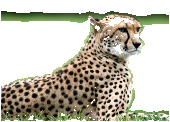
\includegraphics[width=\textwidth]{../output/cheetah4_cropped.png}
        \caption{Cheetah Segmentation with $k=8$}
        \label{fig:CheetahSeg}
	\end{subfigure}
	\begin{subfigure}[b]{0.48\textwidth}
        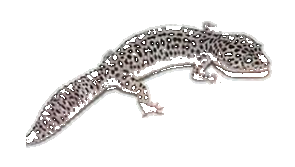
\includegraphics[width=\textwidth]{../output/gecko4_cropped.png}
        \caption{Gecko Segmentation with $k=6$}
        \label{fig:DogSeg}
	\end{subfigure}
\end{figure}

\subsection*{Original vs. Transferred Foreground}

\begin{figure}[H]
	\begin{subfigure}[b]{0.46\textwidth}
        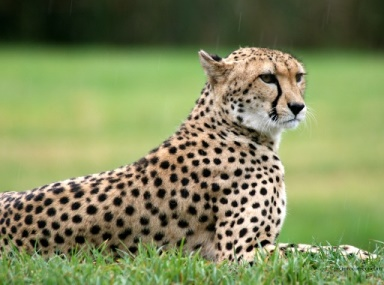
\includegraphics[width=\textwidth]{../images/cheetah.jpg}
        \caption{Original Cheetah}
        \label{fig:Cheetah}
	\end{subfigure}
	\begin{subfigure}[b]{0.54\textwidth}
        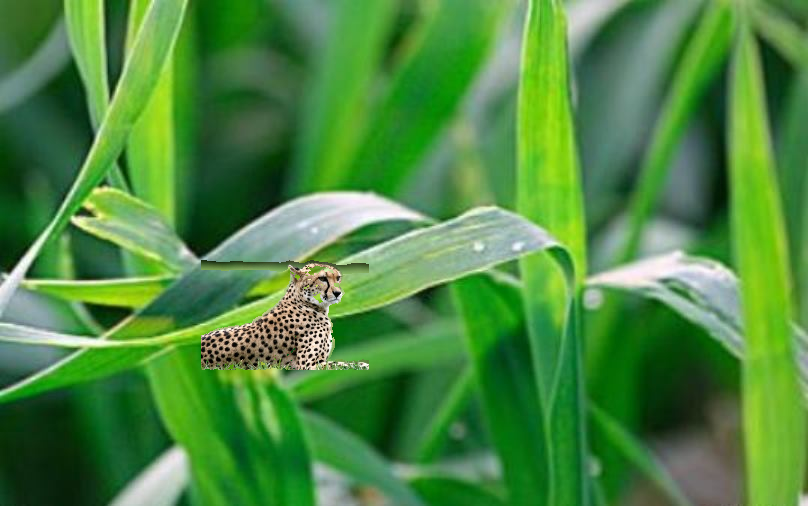
\includegraphics[width=\textwidth]{../output/cheetah2.png}
        \caption{Transferred Cheetah ($k=8$)}
        \label{fig:CheetahTrans}
	\end{subfigure}
\end{figure}

\begin{figure}[H]
	\begin{subfigure}[b]{0.256\textwidth}
        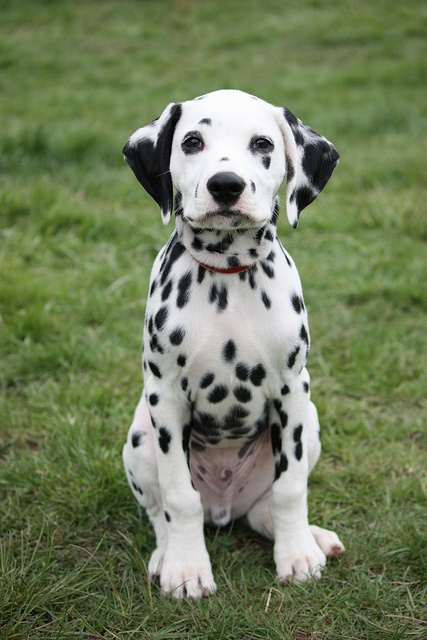
\includegraphics[width=\textwidth]{../images/dog.jpg}
        \caption{Original Dog}
        \label{fig:Dog}
	\end{subfigure}
	\begin{subfigure}[b]{0.7\textwidth}
        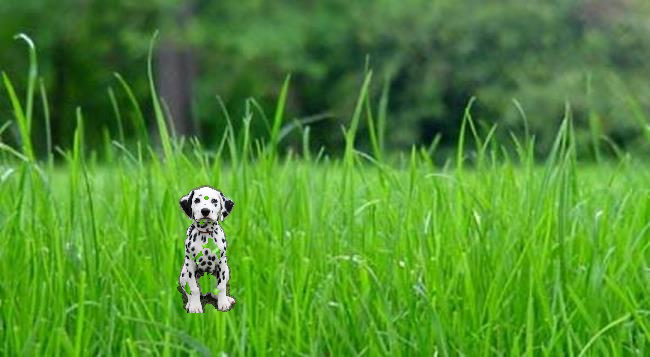
\includegraphics[width=\textwidth]{../output/dog23.png}
        \caption{Transferred Dog ($k=5$)}
        \label{fig:DogTrans}
	\end{subfigure}
\end{figure}

\begin{figure}[H]
	\begin{subfigure}[b]{0.51\textwidth}
        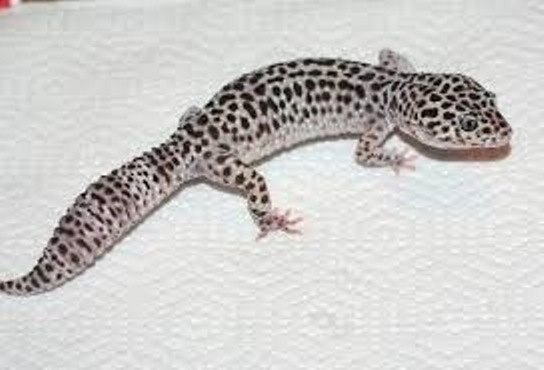
\includegraphics[width=\textwidth]{../images/gecko.jpg}
        \caption{Original Gecko}
        \label{fig:Gecko}
	\end{subfigure}
	\begin{subfigure}[b]{0.49\textwidth}
        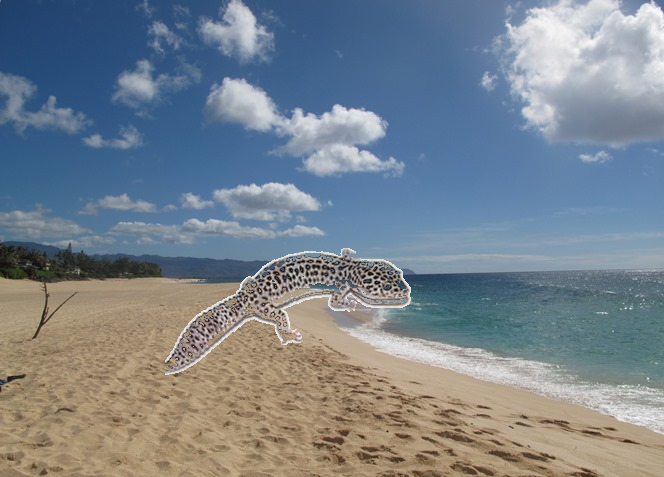
\includegraphics[width=\textwidth]{../output/gecko1.png}
        \caption{Transferred Gecko ($k=6$)}
        \label{fig:GeckoTrans}
	\end{subfigure}
\end{figure}

\begin{figure}[H]
	\begin{subfigure}[b]{0.45\textwidth}
        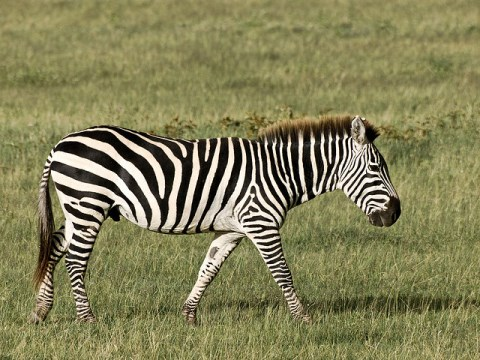
\includegraphics[width=\textwidth]{../images/zebra.jpg}
        \caption{Original Zebra}
        \label{fig:Zebra}
	\end{subfigure}
	\begin{subfigure}[b]{0.55\textwidth}
        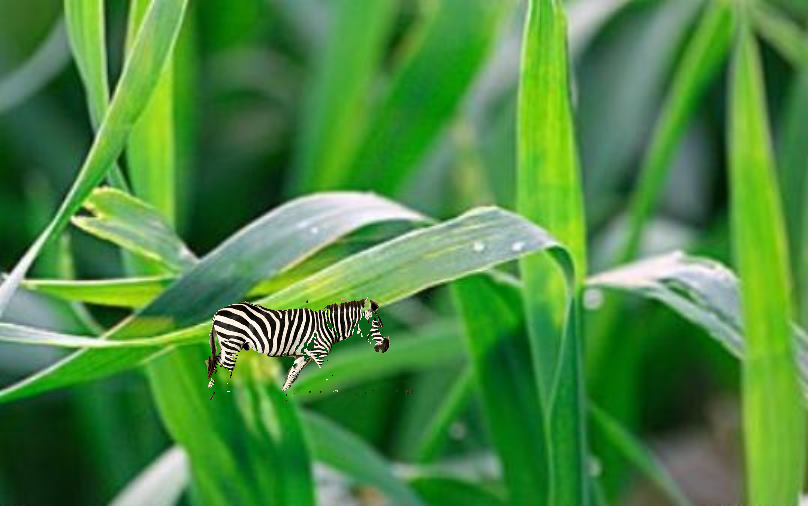
\includegraphics[width=\textwidth]{../output/zebra2_k=4.png}
        \caption{Transferred Zebra ($k=5$)}
        \label{fig:ZebraTrans}
	\end{subfigure}
\end{figure}





\end{document}

